\section{Introduction}

La réalisation des applications téléphoniques nécessitent différentes technologies et d'outils. Les applications Iphone et Android nécessitant des outils différents, une partie non négligeable de mon travail a été de me former sur ceux-ci.

Malgrès la différence de ces deux système d'exploitation, il existe quelques ressemblance, en particulier sur leur utilisation du pattern MVC (Model View Controler).Le modèle s’occupe de stocker les données, la vue les affiche à l’utilisateur, en créant les différents éléments de navigation et d'interaction. Enfin le contrôleur réalise le lien entre la vue et le modèle. Il récupère les informations de la vue, pour les stocker dans le modèle. Le modèle notifie le contrôleur pour que celui-ci mette à jour la vue.

A la suite de plusieurs recherches sur les documentations officielles j'ai pu noter les points suivant pour chacun des systèmes d'exploitation téléphonique.

\section{Technolgie utilisée pour Android}

\subsection{Les outils utilisés}

Pour réaliser des applications Android nous devons utiliser différents outils, que ce soit pour le développement ou pour la mise en production.

\subsubsection{Eclipse}

Eclipse est un IDE (Integrated Development Environment) permettant principalement le développement Java. Android étant réalisé en Java il est possible d'intégrer des plugins permettant le développement d'application Android avec cet IDE. De plus il est nécessaire de détenir le SDK d'Android. Un SDK est un kit de développement pour la réalisation d'application de type défini.

\subsubsection{Le Playstore}

Le Playstore est la plateforme officiel de Google qui permet de mettre à disposition des utilisateurs des applications téléphonique. Cette mise en production est relativement rapide, de l'ordre de quelques heures.

\subsection{Le langage de programmation}

\subsubsection{Activity}

Une activité, au sens Android, est une classe permettant l’interaction avec l'utilisateur. Cette classe gère la création d'une vue ainsi que les actions de l'utilisateur sur cette vue. L'activité passe par plusieurs étapes qui sont représentés sur le schéma suivant.

\begin{figure}[!h]
	\centering
	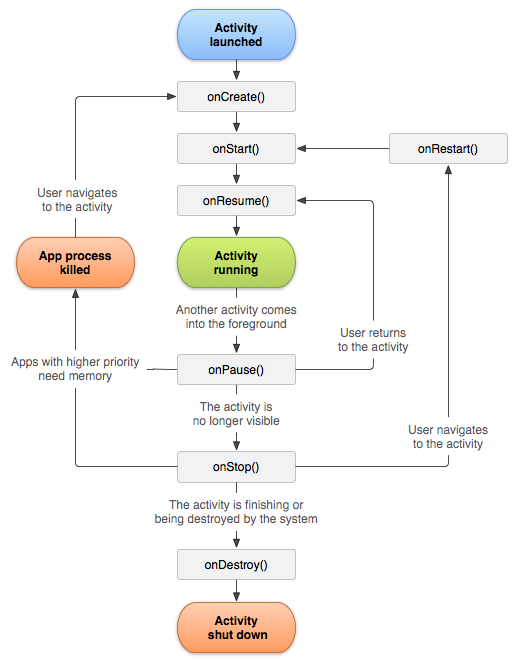
\includegraphics[scale=0.6]{img/activity_lifecycle.png}
	\caption{\label{activity_lifecycle} Cycle de vie d'une activité Android}
\end{figure}

On peut résumer tout ces étapes en quatre états :
\begin{description}
	\item[Active] L'activité est au premier plan et peut être contrôlée par l'utilisateur (onResume -> onPause);
	\item[En pause] L'activité est visible mais les actions de l'utilisateur ne sont plus pris en charge (onPause). Dans cet état toutes les données de l'activité sont conservées, mais en cas de manque de mémoire de la part de l'appareil téléphonique, l'activité est détruite;
	\item[Stoppée] L'activité n'est plus visible elle est stoppée. Elle réagis de la même manière que dans un état de pause en ce qui concerne la mémoire des informations;
	\item[Détruite] L'activité est tuée, toutes ses informations sont effacées de la mémoire.
\end{description}
%%http://developer.android.com/reference/android/app/Activity.html#ActivityLifecycle

\subsubsection{Intent}

L'objet Intent permet le démarrage d'une activité ou d'un service. Un service réagis comme une activité qui n'aurai pas besoin d'interface utilisateur et qui tournerais en arrière plan. Ce démarrage peut être initié par n'importe quel composant de l'application.

\subsubsection{Manifest}
Le fichier Manifest représente les informations essentielles de l'application Android afin de créer le fichier APK nécessaire au lancement de l'application Android. Un fichier APK (Android PacKage) est un paquetage de fichiers compressés pour le système d'exploitation Android.

\section{Technologie utilisée pour IOS}

\subsection{Les outils utilisés}

\subsubsection{Xcode}
Xcode est l’IDE permettant de développer les applications Apple (applications bureautiques et applications mobiles). Xcode est donc l’IDE de choix par défaut pour développer une application iOS. Xcode intègre un simulateur permettant d’émuler les périphériques (iPhone, iPad) de notre choix et d’exécuter l’application sans devoir passer par un périphérique physique bien que cela soit également possible. Pour ma part j'avais à disposition deux Iphones avec différentes version d'Ios afin de tester la compatibilité sur les IOS version 7 et 8. 

\subsubsection{Itunes Connect}
ITunes Connect est un site internet permettant de gérer les applications réalisées auprès d’Apple. Pour une entreprise, une fois enregistrée au programme de développement Apple, ce site permet de définir les membres de l’équipe de développement et leurs rôles au sein de l’équipe. Je possédais les permissions techniques qui permettent de développer des applications et de les publier sur l’Appstore. 

L'Appstore est la plateforme de téléchargement d'applications en ligne d'Apple. ITunes Connect permet aussi de définir l’ensemble des métadonnées qui seront présentées aux utilisateurs lors de leur achat de l’application sur l’AppStore (mots-clés, descriptif, captures d’écrans, prix ..).

Ce site permet également d'avoir un retour sur les utilisateurs de l'application (commentaires, nombre de téléchargements, note obtenue sur l'application ...)


\subsection{Le langage de programmation}

\subsubsection{Delegate}

La délégation permet, comme son nom l'indique, de déléguer des méthodes vers un autre objet. Elle se fait par l'envoi d'un message qui informe le délégué. Le message est ensuite traité par le délégué. Le délégué pourra répondre à ce message en renvoyant un résultat ou en mettant à jour une vue. Le système de délégation a été utilisé afin de faire transiter des informations entre les différentes vues de l'application développée. La délégation s'effectue par la définition d'un protocole décrivant les messages envoyés entre les objets.

Pour définir une délégation, un objet doit hériter d'un objet \textit{delegate}. Cette héritage pourra nécessiter une redéfinition des méthodes voulues par le développeur. Si certaines méthodes ne sont pas redéfinies, alors une méthode par défaut définie dans l'objet \textit{delegate} sera appelée. On peut comparer ce procédé à une interface Java à la différence que toutes les méthodes n'ont pas à être définies.

\subsubsection{Block}

Un \textit{block} permet de définir une fonction, qui pourra être utilisé en tant que paramètre dans une autre méthode ou une autre fonction. Ceci peut être utile lors de l'appel de méthode asynchrone qui nécessite le traitement de données reçues ou le démarrage d'un autre processus.